%%%%%%%%%%%%%%%%%%%%%%%%%%%%%%%%%%%%%%%%%%%%%%%%%%%%%%%%%%%%%%%%%%%%%%%%%%%%%%%%%%%%%%%%%%%%%%%%%%%%%%%%%%%%%%%%%%%%%%
\chapter{Fundamentos en Cosmología }\label{chap:marco}
%%%%%%%%%%%%%%%%%%%%%%%%%%%%%%%%%%%%%%%%%%%%%%%%%%%%%%%%%%%%%%%%%%%%%%%%%%%%%%%%%%%%%%%%%%%%%%%%%%%%%%%%%%%%%%%%%%%%%%

La cosmología es una rama de la física que busca explicar todo lo 
concerniente a la estructura a gran escala en el universo. En este 
marco nos encontramos con problemas muy interesantes como una posible 
explicación del porqué de la estructura filamentaria observada a 
gran escala, la expansión del Universo, la radiación cósmica de fondo, 
la época de reionización, la abundancia de elementos, en especial 
aquellos formados en la nucleosíntesis primordial, entre muchos otros 
tópicos. 

Para lograr dicho cometido es esencial adquirir conocimientos básicos 
de relatividad ge\-ne\-ral, ésta es la teoría hoy en día aceptada para 
estudiar la interacción gravitacional en escalas astronómicas. 
Para su desarrollo fue necesaria la geometría riemanniana, el 
cálculo tensorial y la relatividad especial. 
Valiendonos de ésta es posible proponer módelos cosmológicos que estén 
acordes con las observaciones astronómicas, por lo que en el presente 
capítulo se expone de forma rudimentaria las bases que nos llevan a las 
ecuaciones de Friedmann, las últimas describen la expansión del Universo.
 
Debido a que el Universo contiene radiación, materia y una contribución 
a la energía por parte del vacío es necesario mirar su evolución con el 
redshift, en partícular el comportamiento de la materia en los primeros 
estadios, tanto la materia bariónica como la oscura.  
A partir de esto se puede estudiar la evolución de las perturbaciones iniciales, esto es, 
fluctuaciones de densidad iniciales que dependen del espectro de 
potencias. Pero las fluctuaciones evolucionan de forma diferente de acuerdo
a la edad del Universo entonces se estudia para un regimen lineal dentro del 
que es válido y otro donde es necesario un colapso no lineal de las fluctuaciones.




%&&&&&&&&&&&&&&&&&&&&&&&&&&&&&&&&&&&&&&&&&&&&&&&&&&&&&&&&&&&&&&&&&&&&&&&&&&&&&&&&&&&&&&&&&&&&&&&&&&&&&&&&&&&&&&&&&&&&&&
\section{M\'etrica Robertson Walker}
%&&&&&&&&&&&&&&&&&&&&&&&&&&&&&&&&&&&&&&&&&&&&&&&&&&&&&&&&&&&&&&&&&&&&&&&&&&&&&&&&&&&&&&&&&&&&&&&&&&&&&&&&&&&&&&&&&&&&&&

Lo que podemos observar en la actualidad es un universo altamente homogéneo 
e isotrópico a grandes escalas. Además de la radiación cósmica de fondo 
conocemos que en una época más temprana al desacople de la radiación y materia
las inhomogeneidades encontradas sólo se presentan en escalas muy pequeñas, 
fluctuaciones que contrastan con la densidad de fondo.  
Como consecuencia se han enunciado dos postulados que permiten  una mayor 
simplicidad en el estudio del cosmos, el principio cosmológico y el postulado 
de Weyl. 

\begin{itemize}
\item Principo cosmol\'ogico: \emph{El universo es isotr\'opico y homog\'eneo 
en grandes escalas.}

No sobra hacer un poco de claridad sobre los términos usados, homogéneo se 
refiere a que independientemente de donde ubiquemos el sistema de referencia se 
observará la misma estructura o propiedades del Universo. Por su parte, la
isotropía establece que independiente de la dirección en que se realice una 
observación se deben nuevamente observar las mismas propiedades del Universo. 
En otras palabras, se tiene simetría rotacional y traslacional para el sistema
de referencia escogido. 

En la actualidad dichas características son observables en escalas de mega parsecs
pero ya que el Universo se encuentra en expansión, dicha escala claramente 
va a depender de la época cósmica en partícular. 


\item Postulado de Weyl:\emph{ Establece que las líneas mundo de las galaxias forman 
un conjunto de geodésicas que no se interceptan, excepto en un punto singular en un 
pasado finitio o infinito}. 

Este postulado nos permite definir un conjunto de observadores que se mueven con 
las líneas mundo de las galaxias, en el punto de intersección se pueden sincronizar 
los relojes entre los observadores y así se logra definir un tiempo cósmico. 

A su vez, se puede determinar la distancia hasta una galaxia en un mismo tiempo 
cósmico permitiendo el uso de una métrica para este tiempo.  

\end{itemize}

Además existe otra premisa importante a tener en cuenta en un módelo 
cosmológico, está es la expansión del Universo, la cuál deja fuertes 
consecuencias en la predicción de la evolución de éste, 
que dependerán del contenido de masa y energía total en el Universo. 
Anteriormente se tenía una idea arraigada, que el universo era estático, muestra de 
ello es el módelo cosmológico propuesto por Einstein donde se incluía 
una constante tal que se satisfacíera dicha condición.
Pero fue gracias a observaciones de galaxias cercanas realizadas 
por Edwin Hubble, que se concluyó que las galaxias en su mayoría 
tienen un corrimiento al rojo, en otras palabras, se están alejando 
de nosotros. 
El considerar dicho alejamiento puede llevarnos a una conclusión errónea, 
pensar que nos encontramos en el centro del Universo. 
Conside\-remos entonces tres galaxias tal como se muestra
en la figura \ref{vectores}, si ubicamos el sistema de referencia en 
la galaxia $1$ se satisfacen las siguientes ecuaciones
\begin{eqnarray*}
\vec{v}_2=H_o \vec{r}_2\\
\vec{v}_3=H_o \vec{r}_3
\end{eqnarray*}

que corresponden a la ley encontrada por Hubble, establece que la velocidad 
con la que se alejan las galaxias es proporcional a la distancia que las separa. 
De lo anterior, la velocidad relativa entre las partículas $2$ y $3$ se puede obtener,
$\vec{v}_{23} = \vec{v}_2 -\vec{v}_3 = H_o(\vec{r}_2-\vec{r}_3)$. 	
Pero a partir de la suma vectorial $\vec{r}_3+\vec{r}_{23} = \vec{r}_2$ se obtiene nuevamente 
la ley de Hubble $\vec{v}_{23}=H_o\vec{r_{23}}$.

%**********************************************************************************************************************
\begin{figure}[htbp]
       \centering
               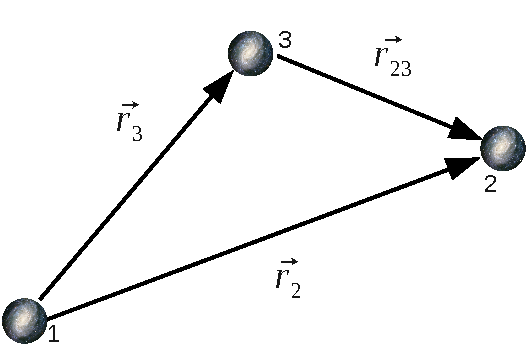
\includegraphics[width=0.43\textwidth]{Images/chapter2/vec.pdf}
       \caption{\small Galaxias que interactuan gravitacionalmente en un Universo 
       homogéneo en expansión.}
       \label{vectores}
 \end{figure}
%**********************************************************************************************************************

Esto es, independiente de donde fijemos el sistema de referencia, 
por ejemplo en la galaxia 3, se observaría nuevamente 
que las galaxias restantes se alejan, lo que nos muestra que no nos encontramos 
en una posición privilegiada. 

\

Con lo expuesto previamente se procede a definir la métrica, 
$ds^2 = g_{\mu\nu}dx^{\mu}dx^{\nu}$, donde $g_{\mu\nu}$ es el 
tensor métrico y $dx^{\alpha}$ denota un desplazamiento infinitesimal 
de las coordenadas $x^{\alpha} = \{ct,x,y,z\}$.  Para que la métrica 
satisfaga las condiciones de isotropía, homogeneidad y expansión, el tensor 
métrico debe tomar la forma $ g_{\mu\nu} = diag\{1,-\frac{a^2}{1-k^2}
-a^2r^2,-a^2r^2\sin^2\theta\}$, de donde la métrica toma la forma

\begin{equation}
ds^2= c^2dt^2-a(t)^2\left[\frac{d^2r}{1-Kr^2} +r^2(d^2\theta
 + \sin^2\theta d^2\phi )\right]
\label{metrica}
\end{equation} 	

esta es conocida como la métrica Robertson Walker. El término $a(t)$ 
es el factor de escala, describe como la distancia relativa entre 
dos observadores fundamentales cambia con el tiempo y $K$ es la 
constante de curvatura en el tiempo actual, define la geometría
del Universo. Lo último se puede ver en más detalle tomando tres
valores para la constante de curvatura, $K=0,\pm 1$. 
Haciendo $K=0$ la expresión \ref{metrica} se reduce a 

\[ds^2= c^2dt^2-a(t)^2\left[d^2r +r^2(d^2\theta + 
\sin^2\theta d^2\phi )\right]\]

que corresponde a la métrica euclideana, en este caso el Universo 
es plano y sufre una expansión constante durante un tiempo indefinido. 
Tomando $K=1$ se obtiene de \ref{metrica}
 
\[ds^2= c^2dt^2-a(t)^2\left[\frac{d^2r}{1-r^2} +r^2(d^2\theta +
\sin^2\theta d^2\phi)\right]\]

que corresponde a una geometr\'ia esf\'erica, el Universo se 
expandiría hasta colapsar nuevamente debido al contenido de masa
y energía de éste. Cuándo se toma $K=-1$

\[ ds^2= c^2dt^2-a(t)^2\left[\frac{d^2r}{1+r^2} +
r^2(d^2\theta + \sin^2\theta d^2\phi)\right]\]

se obtiene una geometr\'ia hiperbólica, el Universo en este 
caso sufre una expansión a\-ce\-le\-ra\-da. Esto se ilustra en la 
figura \ref{factor}. Se debe tener presente que  en realidad
la geometría del Universo  depende del contenido
de materia y energía total en el Universo $\Omega_o$, 
puesto que la constante de curvatura está dada por 
$K = H_o^2(\Omega_o -1)/c^2$. 
 
%**********************************************************************************************************************
\begin{figure}[htbp]
       \centering
               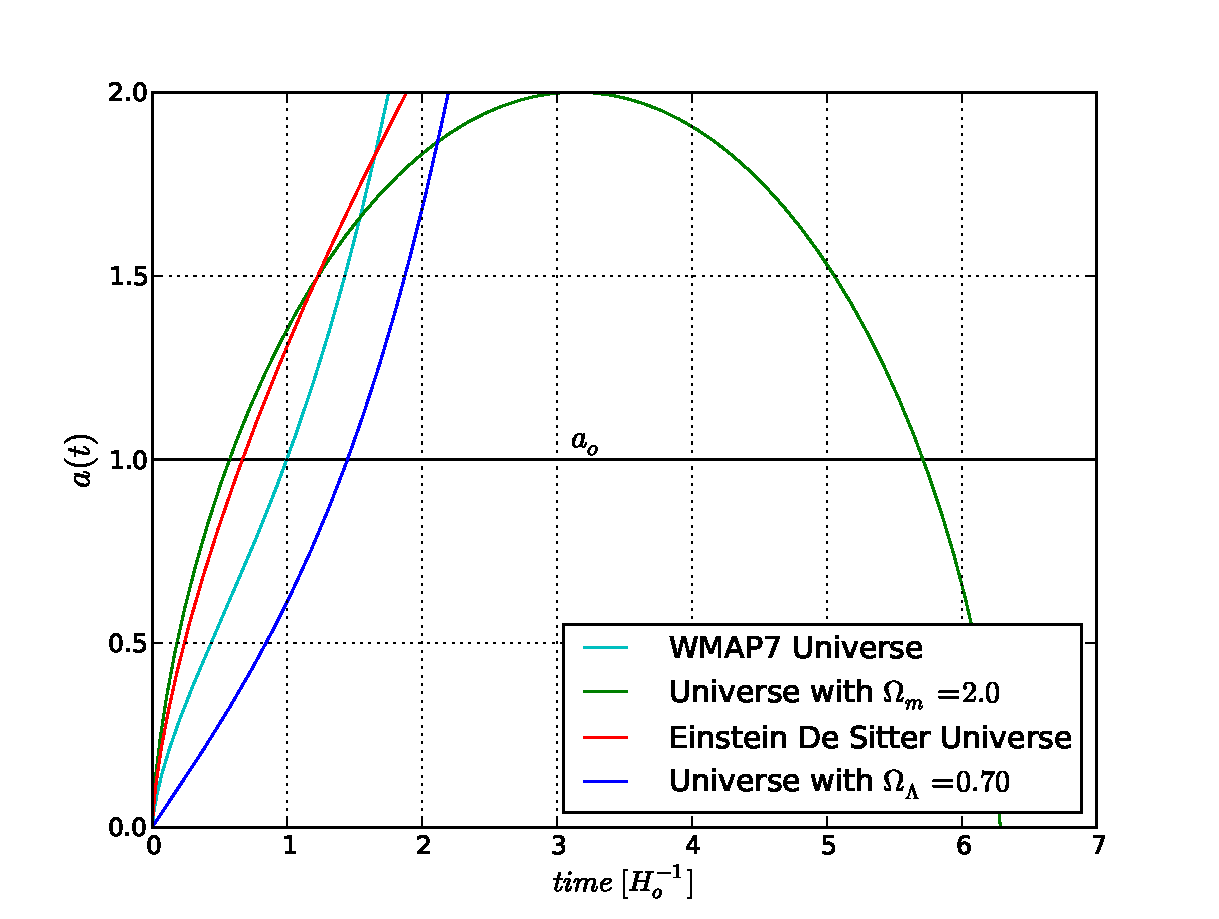
\includegraphics[width=0.8\textwidth]{Images/chapter2/factordeescala.pdf}
       \caption{ \small Factor de Escala en función del tiempo. La expansión del Universo para 
       diferentes contribuciones a la densidad, se obtiene un Universo cerrado para $\Omega_m = \Omega_o>1$,
       los parámetros WMAP7 muestran que el Universo sufre una expansión acelerada. 
       }
       \label{factor}
 \end{figure}
%**********************************************************************************************************************


%&&&&&&&&&&&&&&&&&&&&&&&&&&&&&&&&&&&&&&&&&&&&&&&&&&&&&&&&&&&&&&&&&&&&&&&&&&&&&&&&&&&&&&&&&&&&&&&&&&&&&&&&&&&&&&&&&&&&&&
\section{Ecuaci\'on de Campo de Hilbert-Einstein}
%&&&&&&&&&&&&&&&&&&&&&&&&&&&&&&&&&&&&&&&&&&&&&&&&&&&&&&&&&&&&&&&&&&&&&&&&&&&&&&&&&&&&&&&&&&&&&&&&&&&&&&&&&&&&&&&&&&&&&&

A grandes escalas la interacción fundamental de mayor importancia es 
la gravitacional, por lo que la teoría general de la relatividad 
es una herramienta esencial en el estudio del cosmos. 
Anteriormente se consideraba válida la teoría newtoniana de la gravitación pero 
difiere considerablemente al compararla con la relatividad, 
puesto que el tiempo y el espacio dejan de ser entes absolutos 
además de ser afectados por 
el contenido de energ\'ia y materia presente en el universo. 

En el marco de la teoría newtoniana, la ecuaci\'on de Poisson ofrece una 
relaci\'on entre la segunda derivada del campo y la densidad de materia 
que es la fuente de dicho campo

\[ \nabla^2\Phi=4\pi G\rho\]

a ésta se reduce la ecuación de campo bajo las condiciones de bajas velocidades 
y campo gravitacional débil ($\Phi/c^2<< 1$). 
Pero la ecuación de campo no solo incluye la de Poisson sino además todo lo 
relacionado con la dinámica newtoniana. La ecuación de campo Hilbert-Einstein es 
entonces

\eq{
R_{\mu\nu}-\f{1}{2}g_{\mu\nu}R-g_{\mu\nu}\Lambda = \f{8\pi G}{c^4}T_{\mu\nu}
}

ésta es una ecuaci\'on tensorial de 6 componentes independientes. 
El primer t\'ermino de la izquierda corresponde al tensor de Ricci 
o a segundas derivadas del tensor m\'etrico $g_{\mu\nu}$. 
En el segundo t\'ermino se encuentra el escalar de curvatura 
que define la geometr\'ia. 
En el tercer t\'ermino $\Lambda$ es la constante cosmol\'ogica, 
es asociada a la la densidad con la que contribuye el vacío a 
la densidad total y sería responsable por la expansión acelerada del 
Universo. 
Al lado derecho de la ecuación se encuentra el tensor momentun-energ\'ia 
en la que se incluyen todas las contribuciones de energía y momentum 
como su nombre lo indica.

Es decir que al lado izquierdo se encuentran los t\'erminos que dan 
cuenta por la geometr\'ia del universo mientras que en la derecha 
los relacionados con la distribuci\'on de materia y e\-ner\-gía. 
Por consiguiente se podría afirmar que la geometr\'ia es determinada por 
el contenido de materia-energ\'ia del universo, aunque estrictamente 
hablando el tensor de energ\'ia momentum tambi\'en depende del tensor m\'etrico. 

Existe un caso interesante del tensor energía momentum, 
cuando estamos tratando un fluido perfecto (sin viscocidad), homogéneo
e isotrópico, éste toma la forma 

\[T^{\mu}_{\sigma}= diag\{c^2\rho,-P,-P,-P\}\]

donde $\rho$ es la densidad y P es la presi\'on del fluido. 
Esto muestra que no solo la densidad ocasiona curvatura del 
espacio-tiempo sino tambi\'en la presi\'on. Ya que el Universo se comporta según
el tensor energía momentum mostrado ésta es la forma indicada para 
su estudio.

\

Existen diversas soluciones a la ecuación de Einstein 
pero no muchas en forma analítica, por ejemplo Schwarzschild encontró 
la m\'etrica de un astro est\'atico y con simetría esférica. 
Otra soluci\'on es la m\'etrica de Kerr que corresponde a un astro en 
rotaci\'on con un campo estacionario. 
Claramente la m\'etrica de Robertson-Walker también satisface dichas ecuaciones.

%&&&&&&&&&&&&&&&&&&&&&&&&&&&&&&&&&&&&&&&&&&&&&&&&&&&&&&&&&&&&&&&&&&&&&&&&&&&&&&&&&&&&&&&&&&&&&&&&&&&&&&&&&&&&&&&&&&&&&&
\section{Ecuaciones de Friedmann}
%&&&&&&&&&&&&&&&&&&&&&&&&&&&&&&&&&&&&&&&&&&&&&&&&&&&&&&&&&&&&&&&&&&&&&&&&&&&&&&&&&&&&&&&&&&&&&&&&&&&&&&&&&&&&&&&&&&&&&&

A partir de las ecuación de campo de Einstein y la métrica Robertson-Walker 
es posible proponer módelos cosmológicos que den cuenta por la dinámica observada 
en el Universo. Para alcanzar éste cometido se toman las componentes 
de la ecuación de campo $\beta=\nu= 0$ (componente tiempo-tiempo) y 
$ii=1,2,3$ (componentes espacio-espacio),
a partir de las cuales se hallan

\begin{equation}
\frac{\ddot{a}}{a} = -\frac{4\pi G}{3 }\left( \rho + 3 \f{P}{c^2} \right)+\frac{\Lambda c^2}{3} 
\label{fried1}
\end{equation}

\[
\f{\ddot{a}}{a}+2\f{\dot{a}^2}{a^2}+2\f{c^2 K}{a^2} = 4\pi G\left( \rho-\frac{P}{c^2}\right)+\Lambda c^2
\]

\

donde se ha tenido en cuenta la forma del tensor energía momentum para 
un fluido ideal. Las anteriores son las ecuaciones de Friedmann, dan 
información sobre la dinámica de la expansión del Universo, los términos 
involucrados son,
$a(t)$ el factor de escala y esta normalizado para la época actual
$a(t_o)=1$, $\rho$ es la densidad de radiaci\'on y materia, $P$ es la 
presión total.   
La ecuación \ref{fried1} tiene la forma de una ecuación de fuerzas, 
puede ser deducida parcialmente a partir de mecánica newtoniana sin 
los términos de presión y constante cosmológica. 
Una forma más usada de las anteriores ecuaciones se obtiene al 
manipularlas algebraicamente

\begin{equation}
H(t)=\frac{\dot{a}^2}{a^2}=\frac{8 \pi G}{3}\left(\rho+\frac{\Lambda c^2}{8\pi G}\right) -\frac{Kc^2}{a^2}
\label{fried1}
\end{equation}


la cual se puede interpretar como una ecuación de energía, 
donde el primer término de la derecha es la energía potencial. 
En ésta ecuación se define el parámetro de Hubble, cuando se evalua para la época
actual éste coincide con la constante de Hubble $H(t_o)=H_o = 100h$ Km $s^{-1}$ $Mpc^{-1}$.


Adicionalmente \ref{fried2} puede expresarse en términos de la densidad 
crítica, ésta es la cantidad de materia y energía necesarias para que el 
Universo sea plano, por lo tanto si el Universo tiene una densidad mayor 
colapsaría sobre sí mismo, en cambio si es menor el Universo seguiría 
expandiendose indefinidamente. Ésta se define como 
$\rho_{crit}(t)= 3H(t)^2/8\pi G$.


Dividiendo \ref{fried2} por la constante de Hubble $H_o$ y definiendo 
el parámetro de densidad $\Omega_{i,o} = \rho_{i,o}/\rho_{crit}(t_o)$ con
$i=m,r,\Lambda$ se obtiene 

\begin{equation}
\frac{H^2(z)}{H_o^{2}}=\Omega_{m,o}\left(1+z\right)^3+
\Omega_{r,o}\left(1+z\right)^4+ \Omega_{\Lambda,o} + ( 1-\Omega_o)
\left(1+z\right)
\label{fried2}
\end{equation}

donde $\Omega_o=\Omega_{m,o} +\Omega_{r,o}+\Omega_{\Lambda,o}$ ,
se ha introducido la relación entre el redshift y el factor de escala 
$1+z=1/a$. Se observan las diferentes contribuciones de la densidad al 
parámetro de Hubble, esto es, la densidad de materia, radiación y vacío. 
Cada una contribuye dependiendo de la expansión del Universo, aunque 
la energía del vacío no varía con el redshift.

\

Inicialmente el Universo estaba dominado por radiación, 
durante esta época la radiación estaba acoplada con la materia, 
es decir, la longitud de onda de De Broglie de los electrones es 
comparable a la longitud de onda de la radiación. Por lo anterior 
el camino libre medio de los fotones era despreciable, ocasionando
que el universo fuera opaco. 
Durante éste acople, la temperatura de la radiación es igual a 
la de la materia y corresponde a la de un cuerpo negro. 

Tal como se ve en la grafica \ref{densidad}, a partir de $z=3230$ la materia
se vuelve la mayor contribuci\'on a la densidad del universo y
cuando $z=1100$ la temperatura ha descendido lo suficiente para que 
la tasa de recombinación sea mayor que la de ionización. 
En este caso recombinación se refiere a la formación de átomos neutros, 
lo que permitió el desacople materia radiación.
Pero la última dispersión de la radiación debido a la 
materia aún puede observarse, corresponde a la radiación 
cósmica de fondo, la cual como consecuencia de la expansión del universo 
ha ido enfriandose hasta alcanzar $T$ = $2.7K$. 
  
%**********************************************************************************************************************
\begin{figure}[htbp]
       \centering
               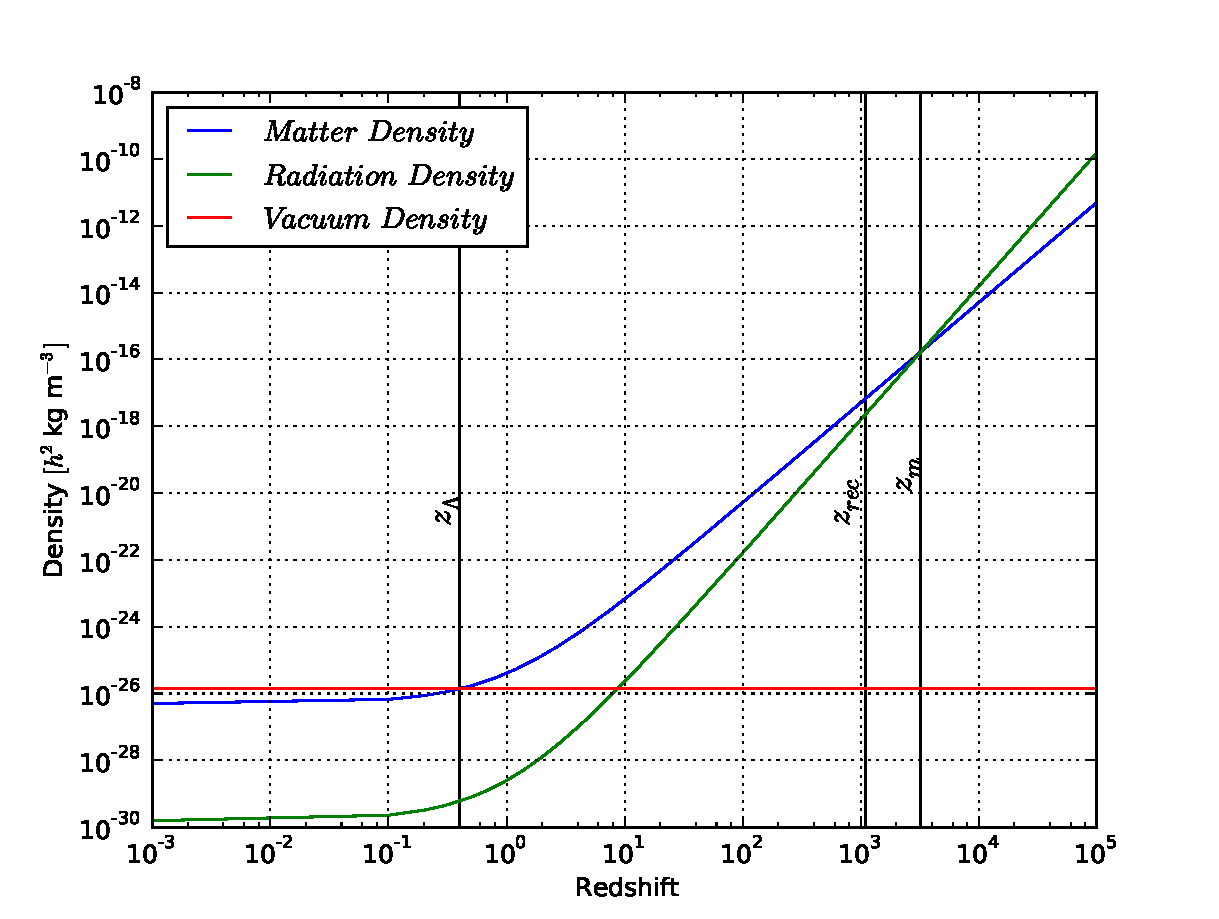
\includegraphics[width=0.8\textwidth]{Images/chapter2/density.pdf}
       \caption{ \small Dependencia en el redshift para $\Omega_\Lambda$, $\Omega_m$ y $\Omega_r$.
       A partir de $z_m$ la densidad de materia domina hasta $z_\Lambda$ 
       donde el término de radiación empieza a dominar. El desacople radiación materia 
       se da para $z_{rec}$. }
       \label{densidad}
 \end{figure}
%**********************************************************************************************************************

En la actualidad el Universo esta dominado por la densidad de vacío, aunque ésta 
es constante puesto que no depende del factor de escala $\rho_{\Lambda}=-c^4\Lambda/8\pi G$,
en contraposición con la materia que depende como $a^{-3}$ y la radiación como $a^{-4}$ 
haciendo que dichas contribuciones disminuyan con el tiempo. 
La constante cosmológica que se observa en esta definición puede ser asociada a una fuerza 
repulsiva que se opone a la gravedad lo que podría dar cuenta de la expansi\'on 
acelerada del universo. 

Existen diversas soluciones a \ref{fried2}, por ejemplo en el Universo Einstein 
de Sitter no existen contribuciones de la radiación o vacío y la densidad total 
es $\Omega_o=1.0$, en este caso la solución toma la forma 

\[
t = \f{2}{3H_o}(1+z)^{-3/2}
\]

y se muestra en \ref{fried2}, donde
dependiendo de los parámetros escogidos cambia la evolución del Universo. En el caso
de WMAP7 los parámetros usados son $\Omega_\Lambda = 0.734$, $\Omega_m = 0.266$(se suman
las contribuciones de materia oscura y bariónica), $\Omega_r = 8.24\times10^{-5}$ y 
$h=0.71$. Éstos últimos son los datos de mayor precisión obtenidos mediante
observaciones de donde se calcula la edad actual del Universo $t\sim 1.2Gyr$. 
Se pueden ver diferentes posibilidades para la evolución
del Universo, por ejemplo, cuando la densidad de materia es la única contribución
y esta es mayor a 1 se obtiene un Universo cerrado. Otro caso es tomar un Universo 
dominado por vacío la densidad necesariamente debe ser $\leq 1$ y es siempre abierto. 
Cuando se tienen las tres contribuciones, el Universo puede ser cerrado o abierto 
dependiendo de cada contribución de los parámetro de densidad y no de la suma total 
aunque $\Omega_o>1$.
	
%&&&&&&&&&&&&&&&&&&&&&&&&&&&&&&&&&&&&&&&&&&&&&&&&&&&&&&&&&&&&&&&&&&&&&&&&&&&&&&&&&&&&&&&&&&&&&&&&&&&&&&&&&&&&&&&&&&&&&&
\section{Ecuaciones de Estado}
%&&&&&&&&&&&&&&&&&&&&&&&&&&&&&&&&&&&&&&&&&&&&&&&&&&&&&&&&&&&&&&&&&&&&&&&&&&&&&&&&&&&&&&&&&&&&&&&&&&&&&&&&&&&&&&&&&&&&&&

Como se ha visto el factor de escala determina la evolución del Universo, 
por consiguiente es importante encontrar las relaciones existentes entre 
dicha cantidad y demás propiedades, se ilustran a continuación algunas 
que se destacan como las más importantes aunque es necesario hacer 
una distinción entre los términos provenientes de la materia, radiación 
y vacío. 

Al asumir que la materia esta en un sistema aislado se conoce
por la primera ley de la termodinámica que satisface $dU = -pdV$, 
en U se incluyen términos relativistas. Haciendo uso del teorema
de equipartición y derivando la energía interna con respecto al factor 
de escala se llega a

\[ T \propto a^{-2} \]

de la ecuación de gas ideal $P = NkT$ y teniendo presente $N = N_oa^{-3}$ 
se conoce además  $P \propto a^{-5}$. La presión debida a la materia
disminuye bastante con la expansión del Universo, mientras 	la densidad 
y la temperatura lo hacen pero de forma menos marcada, otro factor 
para que el vacío domine la expansión del Universo en la actualidad.   

\

La densidad de energía de radiación es

\[\xi=\sum_{\nu}N(\nu)h\nu\]

donde $N(\nu)$ es la densidad de fotones y satisface $N \propto (1+z)^3$,
así que $\xi \propto  \sum_\nu C_\nu a^{-4} $. Comparando con la ley 
de Stefan Boltzmann se concluye $T\propto a^{-1}$.
La dependencia de la presión de radiación en el factor de escala
se halla al recordar que se satisface $ P=\frac{1}{3}\epsilon_{total}$
encontrado que $P \propto a^{-4}$. 

El vacío satisface $\epsilon_{total}=\rho c^2$ donde $\rho$ es una densidad 
efectiva, reemplazando en la primera ley de la termodinámica y derivando 
con respecto al factor de escala se obtiene 

\[ P=-\rho c^2 = -\f{ \Lambda c^4}{8\pi G}\]

para su deducción se tuvo en cuenta la constancia de la densidad.  


%&&&&&&&&&&&&&&&&&&&&&&&&&&&&&&&&&&&&&&&&&&&&&&&&&&&&&&&&&&&&&&&&&&&&&&&&&&&&&&&&&&&&&&&&&&&&&&&&&&&&&&&&&&&&&&&&&&&&&&
\section{Evolución de las Perturbaciones de Densidad en Régimen Newtoniano}
%&&&&&&&&&&&&&&&&&&&&&&&&&&&&&&&&&&&&&&&&&&&&&&&&&&&&&&&&&&&&&&&&&&&&&&&&&&&&&&&&&&&&&&&&&&&&&&&&&&&&&&&&&&&&&&&&&&&&&&

Tal como se mencionó previamente no podemos detectar radiación proveniente 
de una época previa a la de reionización, a causa de la dispersión Compton
que mantenía acopladas la radiación y materia.
Aunque si se puede observar la distribución altamente homogénea de la materia
a este redshift en la radiación cósmica de fondo (Figura \ref{CMB}\footnote{
Imagen WMAP obtenida en \url{http://lambda.gsfc.nasa.gov/product/map/current/m_images.cfm}}).  
Dicha radiación cae en el microondas y da cuenta de variaciones 
en la densidad de fondo, estás últimas resultan ser las causantes de 
la estructura del Universo observada a más pequeñas escalas.
Las variaciones en la densidad son fluctuaciones, $\delta$, que fueron 
incrementando en el transcurso del tiempo, al menos las de nuestro
interes. 
Fue hasta que $\delta\sim 1$  que las fluctuaciones fueron lo 
suficientemente grandes para ser consideradas objetos indi\-vi\-dua\-les, es decir,
su movimiento no solo se debía al flujo de Hubble. 
Lo anterior permite dar una cota superior en redshift a la formación de galaxias, 
que se encuentra alrededor de $z\sim 100$, cuando la densidad promedio de estás 
comparada con las de fondo es aproximadamente $1\times 10^6$. 

Las fluctuaciones iniciales pueden ser tratadas en un regimen líneal mientras 
los contrastes en densidad sean $\delta\ll 1$, por lo que para $z<100$ es una 
suposición razonable. 

%**********************************************************************************************************************
\begin{figure}[htbp]
       \centering
               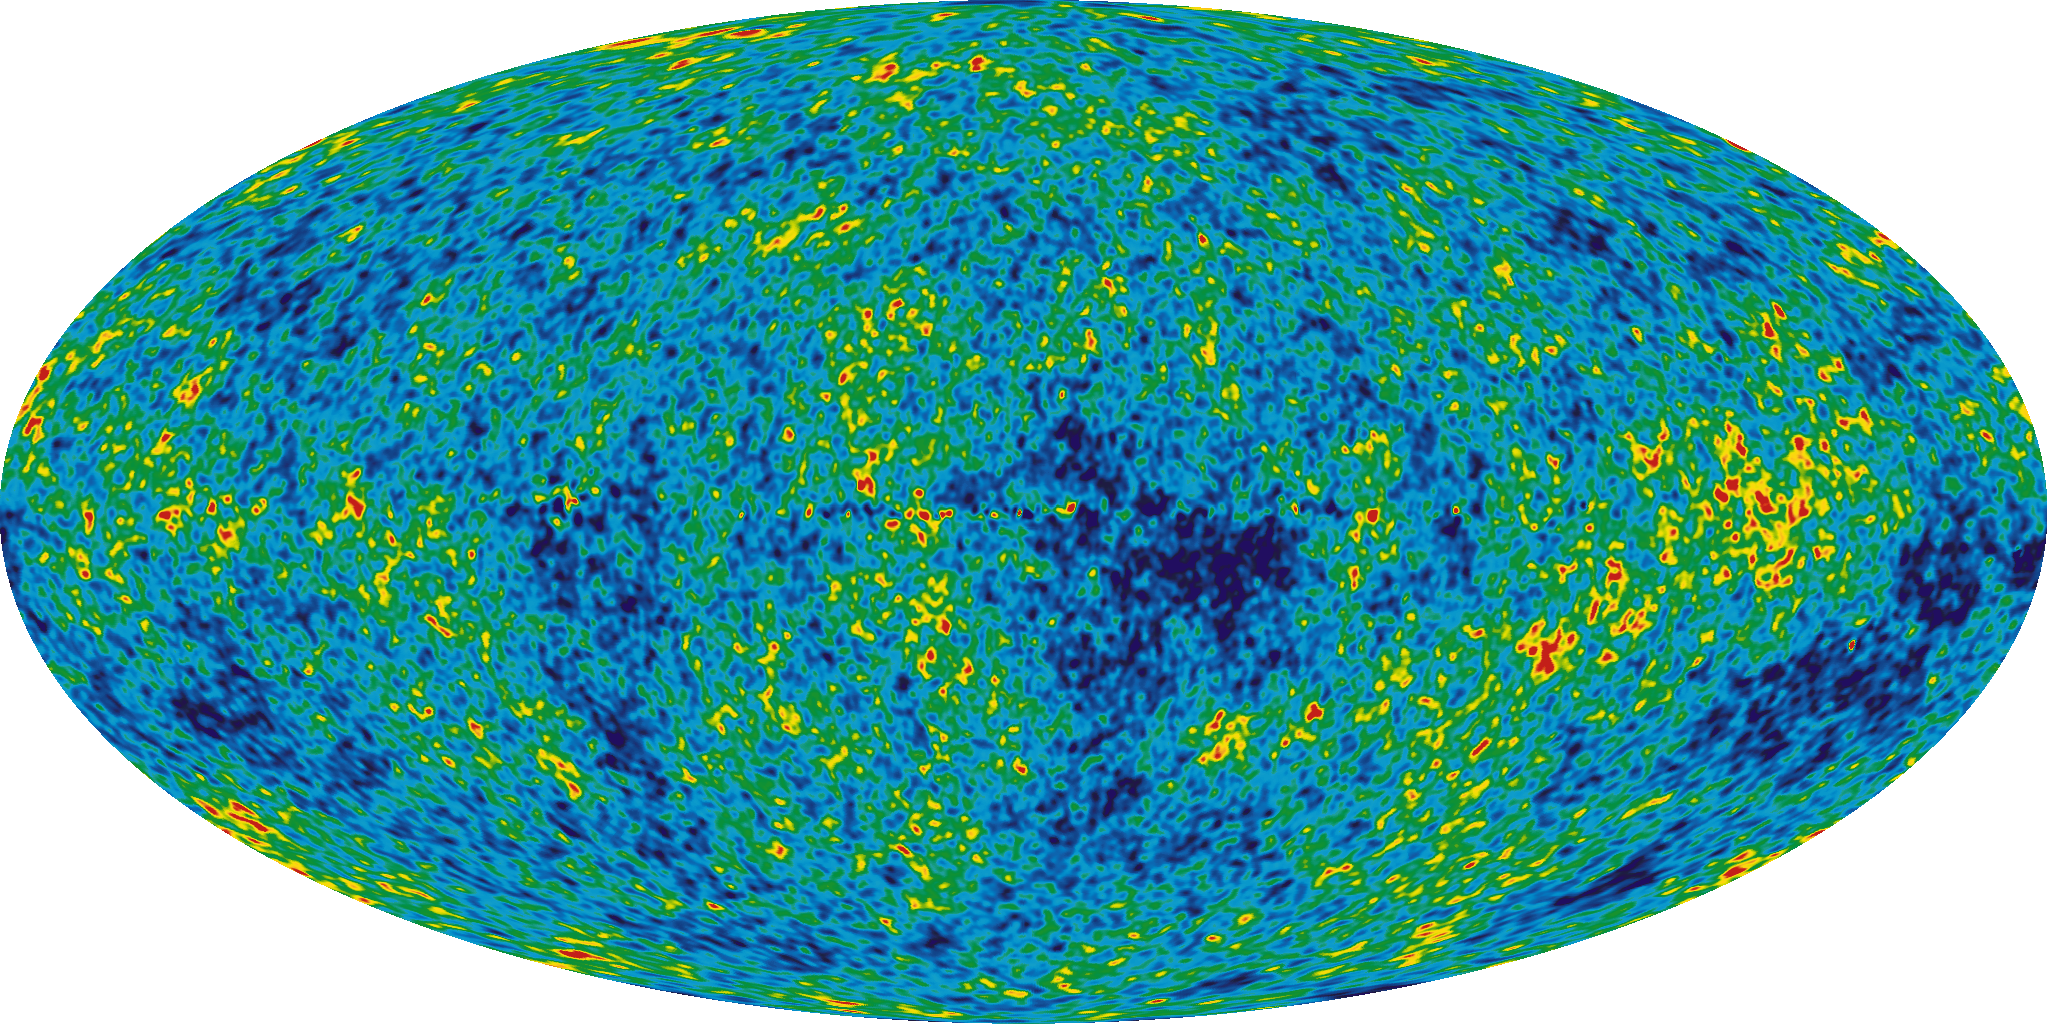
\includegraphics[width=0.6\textwidth]{Images/chapter2/CMB.png}
       \caption{\small Imagen de la radiación cósmica de fondo obtenida por el WMAP,
      que resulta de una combinación de de los 5 mapas obtenidos por dicha sonda. }
       \label{CMB}
 \end{figure}
%**********************************************************************************************************************

%######################################################################################################################
\subsection{Descripción Newtoniana}
%######################################################################################################################

Las fluctuaciones de densidad iniciales tienen una longitud característica mucho menor 
que la distancia de Hubble, la última se define como $d_H \approx ct$. En otras palabras,
el tamaño de las fluctuaciones es muy pequeño comparada con la escala en la que la 
curvatura del Universo es signficativa, permitiendo que la aproximación newtoniana sea válida. 

Por lo tanto, para partículas en movimiento sometidas a un campo gravitacional y cambios 
de presión se satisfacen las siguientes ecuaciones

\begin{eqnarray}
\der{\rho}{t}&=& -\rho \nabla_r\cdot \textbf{u} \nonumber\\
\der{\textbf{u}}{t} &=& -\f{\nabla_r P}{\rho}-\nabla_r\phi \nonumber\\
\nabla^2_r \phi & =& 4\pi G\rho 
\label{euler}
\end{eqnarray}

Como se busca estudiar las fluctuaciones de densidad es útil expresar la 
densidad como $\rho = \overline{\rho}+\delta\rho$, donde $\overline{\rho}$
es la densidad de fondo. Adicionalmente es necesario aclarar que la velocidad 
con la que las partículas se desplazan corresponde a dos contribuciones diferentes, 
la primera es causada por la expansión del Universo y la 
otra es la velocidad propia de la partícula. Partiendo de esto, se
podría pensar en cambiar el sistema de referencia
de las ecuaciones \ref{euler} tal que se satisfaga una descripción lagrangiana, 
esto es, moverse con la expansión del Universo. 
Veamos esto en más detalle, la velocidad en la descripción euleriana está dada 
por $\textbf{u}= a\dot{\textbf{x}}+
\textbf{x}\dot{a} = \textbf{v}+\textbf{x}\dot{a}$, donde $\textbf{v}$ es la velocidad 
peculiar de la partícula y $\textbf{x}\dot{a}$ es la velocidad de expansión del Universo.
Luego, haciendo un cambio a coordenadas comóviles(coordenadas que se mueven con 
la expansión del Universo) y teniendo en cuenta la forma de la densidad se llega al
siguiente conjunto de ecuaciones

\begin{eqnarray}
\pder{\delta}{t} &=& -\f{1}{a}\nabla\cdot[(1+\delta)\textbf{v}]\nonumber\\
\pder{\textbf{v}}{t}+\f{\dot{a}}{a}\textbf{v}+\frac{1}{a}(\textbf{v}\cdot\nabla)\textbf{v}& = &
-\f{\nabla \Phi}{a}-\f{\nabla P}{a\overline{\rho}(1+\delta)}\nonumber\\
\nabla^2 \Phi &=& 4\pi G\overline{\rho}a^2\delta
\label{ec.movimiento}
\end{eqnarray}

la primera corresponde a la ecuación de continuidad, la segunda es la ecuación de 
Euler y la última es la ecuación de campo gravitacional poissoniana. La velocidad
es entonces debida a interacciones gravitacionales y cambios en la presión y $\Phi$ 
es un potencial efectivo. 
Se puede mostrar adicionalmente que la ecuación de estado que relaciona las cantidades
termodinámicas P, $\rho$ y s(entropía) para dicho fluido está dada por 

\begin{equation}
P(\rho,s)= \left[\f{h^2}{2\pi(\mu m_p)^{5/3}}e^{-5/3}\right]\rho^{5/3}\exp \left(\frac{2}{3}\f{\mu m_ps}{k_B}\right)
\label{ec.estado}
\end{equation}

Por medio de la manipulación algebraica de la ecuación de continuidad, la ecuación de Poisson 
incluyendo además la ecuación de estado se haya una ecuación de onda para las fluctuaciones de 
densidad 

\begin{equation}
\f{\partial^2\delta}{\partial t^2}+2\f{\dot{a}}{a}\pder{\delta}{t} =
4\pi G \overline{\rho}\delta + \f{C_s^2}{a^2}\nabla^2\delta+\f{2}{3}\f{\overline{T}}{a^2}\nabla^2s
\label{onda}
\end{equation}

donde $\overline{T}$ es la temperatura del fondo, $C_s$ es la velocidad del sonido. 
Al lado derecho se encuentran las fuentes de las 
fluctuaciones de densidad, como el campo gravitacional, la curvatura dada en términos de la segunda 
derivada de las perturbaciones y cambios en la entropía del sistema. En el lado izquierdo 
se encuentra el parámetro de Hubble que responde por la disipación de la fluctuación debido 
a la expansión del Universo. 

Se propone una solución a la ecuación de perturbaciones en términos de la serie de Fourier 

\begin{eqnarray}
\delta(x,t) &=& \sum_k \delta_k(t)e^{ik\cdot x} \nonumber\\
s(x,t) &=& \sum_k s(t)e^{ik\cdot x} \nonumber
\end{eqnarray}

otro aspecto a tener presente es la independencia de las funciones $e^{ik\cdot x}$ lo que permite expresar 
la ecuación \ref{onda} como

\begin{equation}
\f{d^2\delta_k(t)}{dt^2}+2\f{\dot{a}}{a}\der{\delta_k(t)}{t} = 
\left[4\pi G\overline{\rho}-\f{C_s^2 k^2}{a^2}\right]\delta_k(t)
-\f{2}{3}\f{\overline{T}}{a^2}k^2s_k(t)
\label{ec.modos}
\end{equation}

la solución de está ecuación nos da los coeficientes de expansión de la serie de 
Fourier, obteniendo así el comportamiento de las fluctuaciones de densidad durante
el tiempo en que el régimen newtoniano permanece válido. 

%######################################################################################################################
\subsection{Inestabilidad de Jeans}
%######################################################################################################################

Antes de resolver la ecuación de modos \ref{ec.modos} es importante tener cierta
intuición sobre los fenómenos físicos que están ocurriendo, esto se puede lograr
de forma más sencilla al hacer varias simplificaciones. Consideremos por ejemplo
un Universo estático $\dot{a}=0$ e isentrópico, de donde la ecuación mencionada 
se reduce a 

\[
\f{d^2\delta_k(t)}{dt^2} +
\omega^2\delta_k(t) = 0
\]

con $\omega^2 = C_s^2k^2/a^2-4\pi G\overline{\rho}$. Claramente la solución de la 
ecuación de modos para un Universo estático va a depender del signo que tome 
$\omega$, si $C_s^2k^2/a^2>4\pi G\overline{\rho}$ entonces $\omega$ es positivo 
haciendo que la solución sea oscilatoria, en otras palabras la solución es una 
onda de sonido que no es inestable gravitacionalmente y 
por consiguiente no es de nuestro interés.
Si se satisface $4\pi G\overline{\rho}>C_s^2k^2/a^2$ la solución toma la forma
$\delta_k(t)\propto e^{\Gamma_k t}$, con $\Gamma_k=i\omega_k$ denominada 
taza de crecimiento, en este caso
la perturbación se puede disipar o contraer dependiendo del signo escogido para 
la raíz cuadrada de la frecuencia. Físicamente lo que ocurre es que 
la gravedad tiende a colapsar la fluctuación, aunque el 
gradiente de presión causado por interacciones atómicas 
intenta impedir dicho colapso. Ahora, a partir de la frecuencia 
se puede definir una longitud mínima que deben tener las 
perturbaciones para que se obtenga una solución inestable, 
la cual recibe el nombre de longitud de Jeans $\lambda_J = 2\pi a/k_j$
y satisface $\lambda_J = 2\pi/k_j = C_s(\pi/G\rho)^{1/2}$.
Al escribir la taza de crecimiento términos de $\lambda_J$, 
se concluye que si $\lambda_{pert}>>\lambda_J$ se satisface la 
perturbación si colapsa, donde $\lambda_{pert}$ es la longitud
de la perturbación. 

Como se mostró la longitud de Jeans depende de la velocidad del 
sonido que está definida como 

\[
C_s^2 = \left( \pder{P}{\rho} \right)_s
\]

y a partir de la ecuación de estado \ref{ec.estado} podemos encontrar
la relación que satisface, teniendo además presente que la temperatura de la 
radiación es igual al de la materia para $z \leq z_{eqv}$
debido al acople. Aunque después de la época de recombinación 
cada componente evoluciona de forma independiente. La longitud de Jeans
y la masa de jeans definida como $M_J =  \pi\overline{\rho}_{m,o}\lambda_J^3 $
estan dadas entonces por 

\begin{eqnarray}
\lambda_J \approx 0.01(\Omega_{b,o}h^2)^{-1/2}Mpc\\
M_J \approx 1.5\times 10^5 (\Omega_{b,o}h^2)^{-1/2}M_{\odot}
\end{eqnarray}

Antes de la época de recombinación la velocidad del sonido era
diferente puesto que la presión y densidad 
deben incluir también la contribución de la radiación, 
aún más que la de la materia ya que 
la densidad de radiación dominaba (figura \ref{densidad}). 
La ecuación de estado válida para este rango es $P = c^2\rho_r/3$
y se puede mostrar que el cambio en el orden 
de magnitud entre la longitud y la masa de jeans 
de antes y después de la época de recombinación evaluada para dicha
época es $2.6\times 10^{-5}$  y $1.8\times 10^{-14}$ respectivamente. 
De lo anterior se puede
concluir que el desacople potenció el colapso gravitacional 
al disminuir drásticamente la longitud característica 
mínima requerida para el colapso gravitacional de las perturbaciones.

\

Hasta el momento no se ha hecho alusión a la materia oscura, una componente
de la densidad de materia que contrario a la bariónica no interactua 
con la radiación. Pero ésta si interactua gravitacionalmente con las 
demás partículas, en especial, al hacerlo con las de su misma especie 
se empiezan a crear pozos de potencial gravitacional alrededor de $z\sim 3500$.
En éstos cae materia bariónica, por lo tanto se crean perturbaciones
desde antes del $z_{rec}$. Ahora, como la materia 
bariónica estaba acoplada a la radiación igual esta perturbación
que comenzaba a formarse podía ser disipada, por ejemplo, por 
la ``amortiguación`` de Silk, fenómeno que consiste en la propagación
de fotones en el gas de fotones-materia, por lo que perturbaciones
con una longitud menor que el camino libre medio de los fotones eran disipadas. 
Por lo expuesto, es correcto afirmar que las fluctuaciones se pueden 
expresar como $\delta = \delta_oD(z)$, permitiendo reescribir la ecuación \ref{ec.modos}

\[
\f{d^2D(z)}{dz^2}+\left[ \f{H'(z)}{H(z)} -\f{1}{1+z}\right]\der{D}{z}
= \f{1}{H^2(z)}\left[ \f{4\pi G\overline{\rho}(z)}{(1+z)^2} \right]D(z)
\]

donde se asumió isotropía y se despreció el término que contiene la velocidad
porqué las perturbaciones que nos interesan satisfacen $\lambda_J \ll \lambda$.
De la anterior ecuación se pueden encontrar soluciones analíticas como el Universo
Einstein de Sitter $\delta_k(z)=\delta_o(1+z)^{-1}$, un Universo dominado por 
radiación $\delta_k(z)=\delta_o(1+z)^{-1.22}$ y un Universo dominado por vacío
$\delta_k(z)=\delta_o(1+z)^{-0.58}$. También se pueden encontrar soluciones 
para diferentes contribuciones de la densidad, en la figura \ref{masavacio}
se muestra la evolución de las fluctuaciones para un módelo de Universo
Masa-Vacío, como es de esperarse para densidades más elevadas de materia las 
fluctuaciones crecen más rápido, mientras que las que las que tienen mayor contribución
de vacío, a causa de una expansión acelerada del Universo, necesitan una masa inicial mayor
para empezar a colapsar. Igualmente se debe tener presente que aunque está 
gráfica va hasta $z=0$ la solución es válida mientras $\delta\ll 1$. 


%**********************************************************************************************************************
\begin{figure}[htbp]
       \centering
               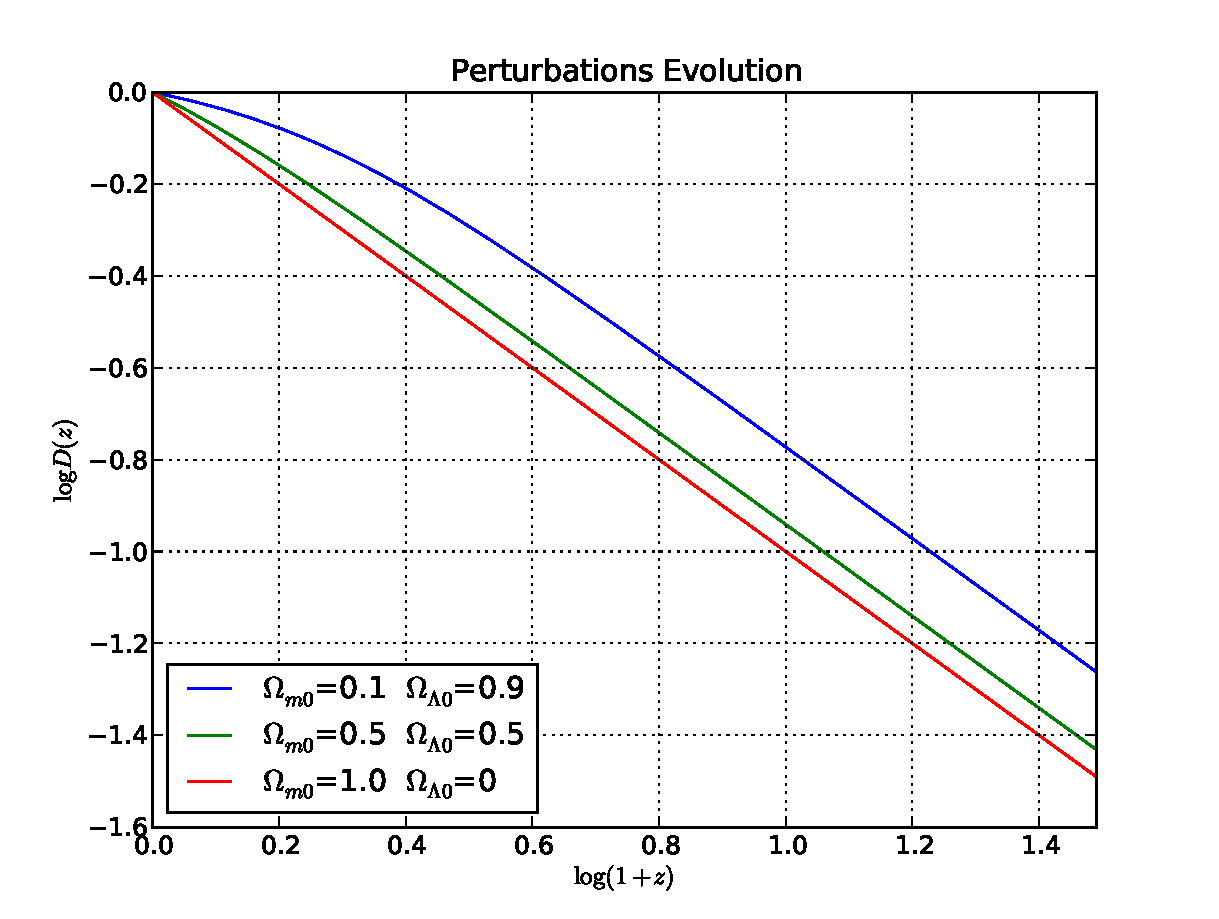
\includegraphics[width=0.8\textwidth]{Images/chapter2/masavacio.pdf}
       \caption{\small Evolución de las perturbaciones para un módelo Masa-Vacío, se muestra el comportamiento
       para diferentes contribuciones de cada componente. }
       \label{masavacio}
 \end{figure}
%**********************************************************************************************************************


%######################################################################################################################
\subsection{Espectro de Potencias}
%######################################################################################################################

Para realizar un estudio del campo de densidad es necesario realizar un 
tratamiento estadístico que nos permita conocer las propiedades de éste. 
En esta dirección, se puede asumir que las fluctuaciones $\delta$ siguen una
distribución normal centrada en $\langle \delta \rangle = 0$, lo cual es soportado
por escenarios inflacionarios que predicen la formación de fluctuaciones como un
campo gaussiano. Entonces, la probabilidad de que 
se tenga un campo de densidad, o dicho en otra forma, la probabilidad de que se tenga 
una distribución específica de fluctuaciones de densidad en el espacio de fourier está
dada por 

\begin{equation}
\mathcal{P}(\delta_{\mbox{\boldmath$\kappa$}})r_{\mbox{\boldmath$\kappa$}}dr_{\mbox{\boldmath$\kappa$}}d\phi_{\mbox{\boldmath$\kappa$}}
=
\exp\left[-\f{r_{\mbox{\boldmath$\kappa$}}^2}{2V_u^{-1}P(\kappa)}\right]	\f{r_{\mbox{\boldmath$\kappa$}}}{V_u^{-1}}
\f{dr_{\mbox{\boldmath$\kappa$}}}{P(\kappa)}\f{d\phi_{\mbox{\boldmath$\kappa$}}}{2\pi}
\label{probabilidad}
\end{equation}

donde los términos dependientes de $r_{\mbox{\boldmath$\kappa$}}$ corresponden a la amplitud de las perturbaciones 
y los de $\phi_{\mbox{\boldmath$\kappa$}}$ a la fase, la última varía aleatoriamente entre $[0,2\pi)$. 
Esta función de densidad de probabilidad conjunta es de utilidad porqué permite independencia en los términos 
$\delta_{\mbox{\boldmath$\kappa$}}$, es decir que es el producto de cada modo 

\[
\mathcal{P}_{\mbox{\boldmath$\kappa$}}(\delta_{\mbox{\boldmath$\kappa$}1},...,\delta_{\mbox{\boldmath$\kappa$}N})=
\prod_{\mbox{\boldmath$\kappa$}}\mathcal{P}_{\mbox{\boldmath$\kappa$}}(\delta_{\mbox{\boldmath$\kappa$}})
\]

lo que no sucede al aplicar la transformada inversa de fourier ya que la función de probabilidad no es separable en el espacio de
coordenadas. El término $P(\kappa)$ en \ref{probabilidad} es el espectro de potencias, éste es definido en el 
espacio de fourier y está relacionada con la función de correlación en el espacio real

\[
P(k) = 4\pi\int_0^\infty \mathcal{E} (r)sinc(kr)r^2dr = V_u  \langle|\delta_{\mbox{\boldmath$\kappa$}}|^2\rangle
\]

$\mathcal{E} (r)$ proporciona la correlación entre dos puntos en el espacio. Adicionalmente se ha encontrado
que el espectro de potencias esperado por la teoría inflacionaría es $P(\kappa)= k^n$, si $n$ toma
el valor de 1 recibe el nombre de espectro Harrison-Zeldovich, es el que mejor 
resultados proporciona. La isotropía del Universo es tomada en cuenta
para el espectro de potencias puesto que se promedia sobre todas las posibles orientaciones del vector 
${\mbox{\boldmath$\kappa$}}$, adicionalmente debe normalizarse con la cantidad $\sigma_8$ que da cuenta
por la amplitud de las fluctuaciones a $8$Mpc/h. 
Cuando el campo se asume como gaussiano se puede mostrar 
que el espectro de potencias contiene toda la información del campo, por lo que
para calcularlo se encuentra el espectro de potencias,
obteniendo la propabilidad de \ref{probabilidad}. Al último se le aplica la transformada inversa
obteniendo así la distribución del campo en coordenadas espaciales. Dicho campo de densidad inicial es usado
para simulaciones cosmológicas o también puede ser tomado de las observaciones realizadas
de la radiación cósmica de fondo. 

%&&&&&&&&&&&&&&&&&&&&&&&&&&&&&&&&&&&&&&&&&&&&&&&&&&&&&&&&&&&&&&&&&&&&&&&&&&&&&&&&&&&&&&&&&&&&&&&&&&&&&&&&&&&&&&&&&&&&&&
\section{Colapso No-lineal de las Perturbaciones de Densidad }
%&&&&&&&&&&&&&&&&&&&&&&&&&&&&&&&&&&&&&&&&&&&&&&&&&&&&&&&&&&&&&&&&&&&&&&&&&&&&&&&&&&&&&&&&&&&&&&&&&&&&&&&&&&&&&&&&&&&&&&

Tal como se mencionó, después de la época de recombinación las fluctuaciones de 
densidad empezaron a crecer, pero la aproximación líneal no es válida para todo
contraste de densidad, por lo que se hace necesario estudiar el crecimiento de
las fluctuaciones cuando $\delta\sim 1$. Aunque solo hasta que la densidad de la 
perturbación alcanza $\sim 100 \overline{\rho}$ es considerada un objeto, dicho en 
otras palabras, la interacción gravitacional determina su dinámica más que la expansión
del flujo de Hubble. El módelo más simple para dar cuenta de dicho fenómeno es 
el de colapso esférico, el escenario considerado es una fluctuación de densidad
que tiene una simetría esférica donde la presión ejercida entre las partículas 
es despreciable. 

A causa de la ausencia de presión, el colapso de la perturbación terminaría 
formando una singularidad, lo cual no sucede como consecuencia
de la presencia de materia oscura y fuerzas de marea. 
La materia oscura permite la formación de regiones más pequeñas
que in\-te\-rac\-tuan causando las fuerzas de marea, 
las regiones finalmente alcanzan equilibrio dinámico y están sometidas 
a un gradiente de potencial gravitacional.
Este proceso recibe nombre de relajación violenta 
y cuando la esfera estudiada finalmente satisface el teorema virial, 
se tiene de la componente de materia oscura un halo dentro del que está embebida 
una galaxia.
Para estudiar dicha formación mediante una simulación cosmológica es necesario hacer 
uso de módelos semianalíticos puesto que la cantidad de partículas involucradas
para dar cuenta de la formación estelar, ratas de supernova, flujos supergalácticos,
entre otros, es inviable computacionalmente, por lo que se usan reglas empíricas
que respondan por dichos fenómenos. 
Retomando el módelo de colapso esférico, el tiempo calculado para que se una 
perturbación colapse está dada por 

\[
1+z_c = \f{1+z_{max}}{2^{2/3}}
\]

donde $z_{max}$ es el tiempo en el que la perturbación se separó de la expansión del Universo. Se nota
que el tiempo de colapso es inferior comparado con el necesario para que la perturbación 
sea un objeto ligado gravitacionalmente. Adicionalmente el estimativo en redshift para que la 
esfera satisfaga el teorema virial es

\[
(1+z_{vir})\leq 0.47\left( \f{v}{100kms^{-1}}\right)^2\left( \f{M}{10^{12}M_{\odot}}\right)^{-2/3}(\Omega_oh^2)^{-1/3}
\]

de donde se nota que para objetos más masivos y con velocidad mayor de dispersión 
el tiempo para que esté virilizado es mucho mayor. 

%######################################################################################################################
\subsection{Aproximación de Zeldovich}
%######################################################################################################################

El módelo anterior para el tratamiento no líneal de las perturbaciones tiene
diversas fallas, la aproximación de Zeldovich aparece como un próximo paso
en una descripción más realista, puesto que, a pesar de asumir un fluido 
sin presión y sin viscosidad considera que la forma de la fluctuación es un
elipsoide. Se parte de que la posición las coordenadas comóviles 
$a(t)\textbf{r}$ satisfacen

\[
\textbf{x} = a(t)\textbf{r}+b(t)\textbf{p}(\textbf{r})
\]

donde $\textbf{r}$ son las coordenadas eulerianas y 
$b(t)\textbf{p}(\textbf{r})$ responde por el desplazamiento con respecto 
a la posición inicial y esta relacionado con el potencial gravitacional 
generado por las fluctuaciones lineales iniciales. 
Se puede mostrar que las perturbaciones estan dadas por 

\[
\rho = \frac{\overline{\rho} }{[1-\alpha b(t)][a(t)-\beta b(t)][a(t)-\gamma b(t)]}a^3(t)
\]

donde $\alpha$, $\beta$ y $\gamma$ dan la contracción o expansión a lo largo de 
los 3 ejes principales del elipsoide. Cuando se satisface $\alpha \geq \beta \geq \gamma$
y $b(t)$ es suficientemente grande aparece una singularidad. Si $\alpha$ además alcanza su máximo 
valor, ocasiona que la fluctuación tome una forma de panqueque por una contracción 
más rápida en el eje x.
A pesar de la simplicidad, el módelo es preciso y esta acorde con los resultados numéricos,
por lo que usado en cosmología observacional y la construcción de condiciones iniciales en 
una simulación N cuerpos.

%&&&&&&&&&&&&&&&&&&&&&&&&&&&&&&&&&&&&&&&&&&&&&&&&&&&&&&&&&&&&&&&&&&&&&&&&&&&&&&&&&&&&&&&&&&&&&&&&&&&&&&&&&&&&&&&&&&&&&&
\section{ Cosmic density field }
%&&&&&&&&&&&&&&&&&&&&&&&&&&&&&&&&&&&&&&&&&&&&&&&&&&&&&&&&&&&&&&&&&&&&&&&&&&&&&&&&&&&&&&&&&&&&&&&&&&&&&&&&&&&&&&&&&&&&&&
%######################################################################################################################
\subsection{ Correlation functions }
%######################################################################################################################
%######################################################################################################################
\subsection{ Mass moments }
%######################################################################################################################
%######################################################################################################################
\subsection{ Clustering in the real and redshift space }
%######################################################################################################################
%-----------------------------------------------------------------------------------------------------------
\subsubsection{ Redshift distortions }
%-----------------------------------------------------------------------------------------------------------
%-----------------------------------------------------------------------------------------------------------
\subsubsection{ Real space correlation functions }
%-----------------------------------------------------------------------------------------------------------

%&&&&&&&&&&&&&&&&&&&&&&&&&&&&&&&&&&&&&&&&&&&&&&&&&&&&&&&&&&&&&&&&&&&&&&&&&&&&&&&&&&&&&&&&&&&&&&&&&&&&&&&&&&&&&&&&&&&&&&
\section{ Baryonic acoustic oscillations }
%&&&&&&&&&&&&&&&&&&&&&&&&&&&&&&&&&&&&&&&&&&&&&&&&&&&&&&&&&&&&&&&&&&&&&&&&&&&&&&&&&&&&&&&&&&&&&&&&&&&&&&&&&&&&&&&&&&&&&&
 